\vspace*{4mm}
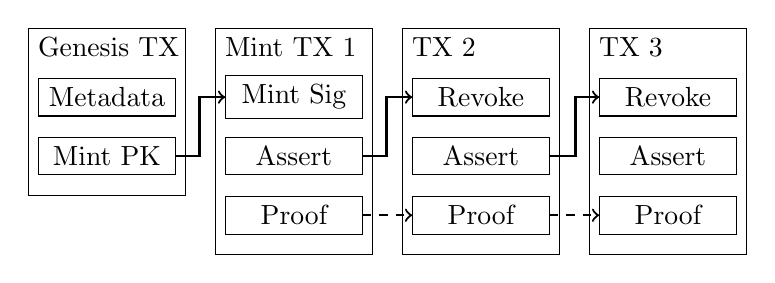
\begin{tikzpicture}
% \node at (-1, 2.5) {Inputs};
% \node at (5, 2.5) {Outputs};

\draw (0, 0.75) rectangle (2,2.875);
\node[below right] at (0, 2.875) {Genesis TX};
\node[draw, text width=1.5cm, align=center] (Metadata 1) at (1,2) {Metadata};
\node[draw, text width=1.5cm, align=center] (Mint PK 1) at (1,1.25) {Mint PK};

\draw (2.375, 0) rectangle (4.375,2.875);
\node[below right] at (2.375, 2.875) {Mint TX 1};
\node[draw, text width=1.5cm, align=center] (Mint Sig 1) at (3.375,2) {Mint Sig};
\node[draw, text width=1.5cm, align=center] (Assert 1) at (3.375,1.25) {Assert};
\node[draw, text width=1.5cm, align=center] (Proof 2) at (3.375,0.5) {Proof};

\draw (4.75, 0) rectangle (6.75,2.875);
\node[below right] at (4.75, 2.875) {TX 2};
\node[draw, text width=1.5cm, align=center] (Revoke 1) at (5.75,2) {Revoke};
\node[draw, text width=1.5cm, align=center] (Assert 2) at (5.75,1.25) {Assert};
\node[draw, text width=1.5cm, align=center] (Proof 3) at (5.75,0.5) {Proof};

\draw (7.125, 0) rectangle (9.125,2.875);
\node[below right] at (7.125, 2.875) {TX 3};
\node[draw, text width=1.5cm, align=center] (Revoke 2) at (8.125,2) {Revoke};
\node[draw, text width=1.5cm, align=center] (Assert 3) at (8.125,1.25) {Assert};
\node[draw, text width=1.5cm, align=center] (Proof 4) at (8.125,0.5) {Proof};

\draw[->, thick] (Mint PK 1) -| (2.175, 2) |- (Mint Sig 1);
\draw[->, thick, dashed] (Proof 2) -- (Proof 3);
\draw[->, thick] (Assert 1) -| (4.55, 2) |- (Revoke 1);
\draw[->, thick] (Assert 2) -| (6.95, 2) |- (Revoke 2);
\draw[->, thick, dashed] (Proof 3) -- (Proof 4);
\end{tikzpicture}
\vspace*{4mm}